\begin{figure}[tbp]
\centering
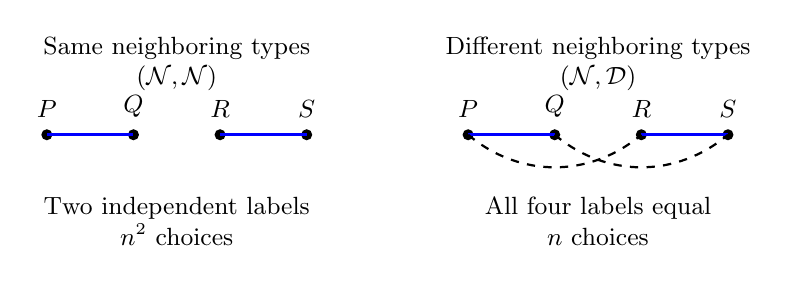
\begin{tikzpicture}[x=1cm,y=1cm,every node/.style={font=\small}]
  \node[align=center] at (1.65,1.65) {Same neighboring types\\($\mathcal N,\mathcal N$)};
  \node[align=center] at (7.0,1.65) {Different neighboring types\\($\mathcal N,\mathcal D$)};
  \foreach \x/\name in {0/P,1.1/Q,2.2/R,3.3/S,5.35/P,6.45/Q,7.55/R,8.65/S} {
    \fill (\x,0.75) circle (2pt);
    \node[above] at (\x,0.85) {$\name$};
  }
  \draw[very thick,blue] (0,0.75) -- (1.1,0.75);
  \draw[very thick,blue] (2.2,0.75) -- (3.3,0.75);
  \draw[very thick,blue] (5.35,0.75) -- (6.45,0.75);
  \draw[very thick,blue] (7.55,0.75) -- (8.65,0.75);
  \draw[thick,dashed] (5.35,0.75) to[bend right=40] (7.55,0.75);
  \draw[thick,dashed] (6.45,0.75) to[bend right=40] (8.65,0.75);
  \node[align=center] at (1.65,-0.35) {Two independent labels\\$n^2$ choices};
  \node[align=center] at (7.0,-0.35) {All four labels equal\\$n$ choices};
\end{tikzpicture}
\caption{Equality constraints on the four path labels at one internal
vertex after the $\mathcal D$ inequalities are relaxed.  Type $\mathcal N$ pairs $P,Q$
and $R,S$ (solid edges); type $\mathcal D$ pairs $P,R$ and $Q,S$ (dashed edges).
Equal neighboring types leave two free labels.  A change of type
identifies all four, contributing a factor $n^{-1}$ to the count.
The same two-label count holds for neighboring types $\mathcal D,\mathcal D$.}
\label{fig:pairings}
\end{figure}
